\section{Lab 2}
\label{sec:lab2}
For the second part of the lab the task is to parallelize a serial implementation of the Red-Back Gauss-Seidal algorithm. This is done using OpenMP (Open \textbf Multi-\textbf Processing) which is an API for forming multi-threaded programs in C, C++, and Fortran. This parallel version is evaluated using the same simulator and CCP:s as in \nameref{sec:lab1}. 

\subsection{Task 1}
The program reads a matrix on the form $n \times n$ containing data points from a file. To make the program simpler and avoid special cases a padding is added to the matrix changing its dimensions to $(n+2) \times (n+2)$. Then every other data point, here by called red dots, is looped through. For every red dot an average of itself and its neighbors to the west, south, north, and east is calculated and written as the dots new value. For all the other data points, called black dots, the same thing is performed. The difference of the dots new and old value is added together and the process is repeated until this accumulated difference of averages, divided by $n^2$, is smaller than $0.01$. After the program finishes its execution the matrix have converged to an average of all red and black dots.

The distribution of the red and black dots forms a chess pattern. This means that when we calculate the average for a dot and its neighbors, all the neighbors are of the other color. As such, when going through for example the red dots there is no need to invalidate any other dots because the black dots are only read and you are the only one accessing your red dot.

\subsection{Task 2}
\label{subsec:lab2:task2}
In listing~\ref{lst:solve} a parallelized version of the function \texttt{void Solve(double **A)} are shown. The parallelization have been done using directives from the OpenMP API. Only this function is shown as the other parts of the program for reading the input file and printing to the console is not included in the performance analysis. The approach taken for making the function execute in parallel is to distribute the lines of the matrix evenly between all threads. This is done twice, once for the red dots and once for the black. Only one thread resets \texttt{diff} to zero on line 5 and test whether the program is finished or not on line 25. At each for loop that goes through the red and black dots the directive \texttt{reduction(+:diff)} is used which causes each thread to have its own private version of \texttt{diff} that all gets added together after the for loop.

\subsection{Task 3}
To be able to evaluate the program described in \nameref{subsec:lab2:task2} we decide to mimic the working set sizes in \nameref{sec:lab1}. However, the provided data files does not include a matrix big enough to fill neither each threads L1 cache or the LLC cache.

In \reffig{fig:lab2} results from running the parallelized version of the program in the simulator with different CCP:s and different matrix dimensions are shown. It can be seen that using MESI over MSI does not cause any noticeable boost in performance. This is because the gain of the extra E state becomes of no importance as the cache lines is in the M state most of the time. Some benefit of the E state can though be seen in Table~\ref{tbl:lab2} as the amount of \textit{WriteMisses} and \textit{InvalidationsSent} are a bit lower for MESI than MSI and the gap becomes bigger as the matrix size increases. This does not show in \reffig{fig:lab2} as the cycle count are not dominated by \textit{WriteMisses} and \textit{InvalidationsSent}.

Changing to MESI-MG yields a huge performance degradation of 420\%, 394\%, and 430\% for matrix size 25, 100, and 200 respectively. This comes from the sharing performed of the brim lines between threads. For each read of a dot in any of these lines, the dot gets migrated over to the thread performing the read. This frequent migration of dots generates a large amount of \textit{ReadMissesSerivcedByModfied} as can be seen in Table~\ref{tbl:lab2}. The overhead stays fairly constant compared to the other CCP:s when the matrix size increases. This is duo to the proportion of sharing between the threads stays the same.  

\begin{figure}[t]
	\center
	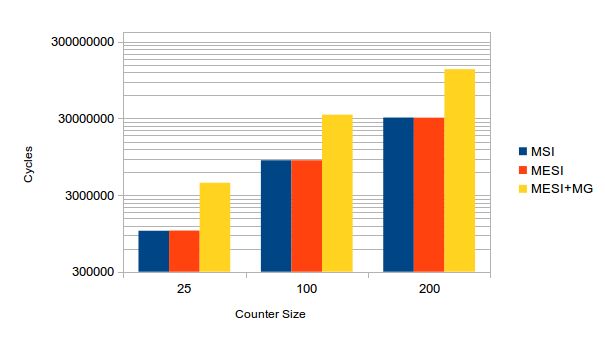
\includegraphics[width=0.8\textwidth]{lab2bars}
	\caption{Results from simulation of the parallelized benchmark for all cache coherence protocols combined with different working sets.}
	\label{fig:lab2}
\end{figure}

\subsection{Task 4}
\todo[inline]{
Outline a strategy to modify the MESI protocol to support the O state.
Analyze the MESI\_SMPCache.cpp source to understand how the MESI protocol is currently modeled.
Discuss changes that need to be made to the readLine, writeLine, readRemoteAction, and writeRemoteAction functions. Show the necessary changes in pseducode. Should the code that tracks cache access statistics be modified? If so, how?}
